% Options for packages loaded elsewhere
\PassOptionsToPackage{unicode}{hyperref}
\PassOptionsToPackage{hyphens}{url}
%
\documentclass[
  man]{apa6}
\usepackage{amsmath,amssymb}
\usepackage{lmodern}
\usepackage{iftex}
\ifPDFTeX
  \usepackage[T1]{fontenc}
  \usepackage[utf8]{inputenc}
  \usepackage{textcomp} % provide euro and other symbols
\else % if luatex or xetex
  \usepackage{unicode-math}
  \defaultfontfeatures{Scale=MatchLowercase}
  \defaultfontfeatures[\rmfamily]{Ligatures=TeX,Scale=1}
\fi
% Use upquote if available, for straight quotes in verbatim environments
\IfFileExists{upquote.sty}{\usepackage{upquote}}{}
\IfFileExists{microtype.sty}{% use microtype if available
  \usepackage[]{microtype}
  \UseMicrotypeSet[protrusion]{basicmath} % disable protrusion for tt fonts
}{}
\makeatletter
\@ifundefined{KOMAClassName}{% if non-KOMA class
  \IfFileExists{parskip.sty}{%
    \usepackage{parskip}
  }{% else
    \setlength{\parindent}{0pt}
    \setlength{\parskip}{6pt plus 2pt minus 1pt}}
}{% if KOMA class
  \KOMAoptions{parskip=half}}
\makeatother
\usepackage{xcolor}
\usepackage{graphicx}
\makeatletter
\def\maxwidth{\ifdim\Gin@nat@width>\linewidth\linewidth\else\Gin@nat@width\fi}
\def\maxheight{\ifdim\Gin@nat@height>\textheight\textheight\else\Gin@nat@height\fi}
\makeatother
% Scale images if necessary, so that they will not overflow the page
% margins by default, and it is still possible to overwrite the defaults
% using explicit options in \includegraphics[width, height, ...]{}
\setkeys{Gin}{width=\maxwidth,height=\maxheight,keepaspectratio}
% Set default figure placement to htbp
\makeatletter
\def\fps@figure{htbp}
\makeatother
\setlength{\emergencystretch}{3em} % prevent overfull lines
\providecommand{\tightlist}{%
  \setlength{\itemsep}{0pt}\setlength{\parskip}{0pt}}
\setcounter{secnumdepth}{-\maxdimen} % remove section numbering
% Make \paragraph and \subparagraph free-standing
\ifx\paragraph\undefined\else
  \let\oldparagraph\paragraph
  \renewcommand{\paragraph}[1]{\oldparagraph{#1}\mbox{}}
\fi
\ifx\subparagraph\undefined\else
  \let\oldsubparagraph\subparagraph
  \renewcommand{\subparagraph}[1]{\oldsubparagraph{#1}\mbox{}}
\fi
\newlength{\cslhangindent}
\setlength{\cslhangindent}{1.5em}
\newlength{\csllabelwidth}
\setlength{\csllabelwidth}{3em}
\newlength{\cslentryspacingunit} % times entry-spacing
\setlength{\cslentryspacingunit}{\parskip}
\newenvironment{CSLReferences}[2] % #1 hanging-ident, #2 entry spacing
 {% don't indent paragraphs
  \setlength{\parindent}{0pt}
  % turn on hanging indent if param 1 is 1
  \ifodd #1
  \let\oldpar\par
  \def\par{\hangindent=\cslhangindent\oldpar}
  \fi
  % set entry spacing
  \setlength{\parskip}{#2\cslentryspacingunit}
 }%
 {}
\usepackage{calc}
\newcommand{\CSLBlock}[1]{#1\hfill\break}
\newcommand{\CSLLeftMargin}[1]{\parbox[t]{\csllabelwidth}{#1}}
\newcommand{\CSLRightInline}[1]{\parbox[t]{\linewidth - \csllabelwidth}{#1}\break}
\newcommand{\CSLIndent}[1]{\hspace{\cslhangindent}#1}
\ifLuaTeX
\usepackage[bidi=basic]{babel}
\else
\usepackage[bidi=default]{babel}
\fi
\babelprovide[main,import]{english}
% get rid of language-specific shorthands (see #6817):
\let\LanguageShortHands\languageshorthands
\def\languageshorthands#1{}
% Manuscript styling
\usepackage{upgreek}
\captionsetup{font=singlespacing,justification=justified}

% Table formatting
\usepackage{longtable}
\usepackage{lscape}
% \usepackage[counterclockwise]{rotating}   % Landscape page setup for large tables
\usepackage{multirow}		% Table styling
\usepackage{tabularx}		% Control Column width
\usepackage[flushleft]{threeparttable}	% Allows for three part tables with a specified notes section
\usepackage{threeparttablex}            % Lets threeparttable work with longtable

% Create new environments so endfloat can handle them
% \newenvironment{ltable}
%   {\begin{landscape}\centering\begin{threeparttable}}
%   {\end{threeparttable}\end{landscape}}
\newenvironment{lltable}{\begin{landscape}\centering\begin{ThreePartTable}}{\end{ThreePartTable}\end{landscape}}

% Enables adjusting longtable caption width to table width
% Solution found at http://golatex.de/longtable-mit-caption-so-breit-wie-die-tabelle-t15767.html
\makeatletter
\newcommand\LastLTentrywidth{1em}
\newlength\longtablewidth
\setlength{\longtablewidth}{1in}
\newcommand{\getlongtablewidth}{\begingroup \ifcsname LT@\roman{LT@tables}\endcsname \global\longtablewidth=0pt \renewcommand{\LT@entry}[2]{\global\advance\longtablewidth by ##2\relax\gdef\LastLTentrywidth{##2}}\@nameuse{LT@\roman{LT@tables}} \fi \endgroup}

% \setlength{\parindent}{0.5in}
% \setlength{\parskip}{0pt plus 0pt minus 0pt}

% Overwrite redefinition of paragraph and subparagraph by the default LaTeX template
% See https://github.com/crsh/papaja/issues/292
\makeatletter
\renewcommand{\paragraph}{\@startsection{paragraph}{4}{\parindent}%
  {0\baselineskip \@plus 0.2ex \@minus 0.2ex}%
  {-1em}%
  {\normalfont\normalsize\bfseries\itshape\typesectitle}}

\renewcommand{\subparagraph}[1]{\@startsection{subparagraph}{5}{1em}%
  {0\baselineskip \@plus 0.2ex \@minus 0.2ex}%
  {-\z@\relax}%
  {\normalfont\normalsize\itshape\hspace{\parindent}{#1}\textit{\addperi}}{\relax}}
\makeatother

% \usepackage{etoolbox}
\makeatletter
\patchcmd{\HyOrg@maketitle}
  {\section{\normalfont\normalsize\abstractname}}
  {\section*{\normalfont\normalsize\abstractname}}
  {}{\typeout{Failed to patch abstract.}}
\patchcmd{\HyOrg@maketitle}
  {\section{\protect\normalfont{\@title}}}
  {\section*{\protect\normalfont{\@title}}}
  {}{\typeout{Failed to patch title.}}
\makeatother

\usepackage{xpatch}
\makeatletter
\xapptocmd\appendix
  {\xapptocmd\section
    {\addcontentsline{toc}{section}{\appendixname\ifoneappendix\else~\theappendix\fi\\: #1}}
    {}{\InnerPatchFailed}%
  }
{}{\PatchFailed}
\keywords{Classical Test Theory, Item Response Theory, item difficulty, item discrimination\newline\indent Word count: X}
\DeclareDelayedFloatFlavor{ThreePartTable}{table}
\DeclareDelayedFloatFlavor{lltable}{table}
\DeclareDelayedFloatFlavor*{longtable}{table}
\makeatletter
\renewcommand{\efloat@iwrite}[1]{\immediate\expandafter\protected@write\csname efloat@post#1\endcsname{}}
\makeatother
\usepackage{csquotes}
\ifLuaTeX
  \usepackage{selnolig}  % disable illegal ligatures
\fi
\IfFileExists{bookmark.sty}{\usepackage{bookmark}}{\usepackage{hyperref}}
\IfFileExists{xurl.sty}{\usepackage{xurl}}{} % add URL line breaks if available
\urlstyle{same} % disable monospaced font for URLs
\hypersetup{
  pdftitle={Classical Test Theory Item Characteristic Curve Estimation: p-value to b-parameter Scaling},
  pdfauthor={Diego Figueiras1 \& John T. Kulas1},
  pdflang={en-EN},
  pdfkeywords={Classical Test Theory, Item Response Theory, item difficulty, item discrimination},
  hidelinks,
  pdfcreator={LaTeX via pandoc}}

\title{Classical Test Theory Item Characteristic Curve Estimation: p-value to b-parameter Scaling}
\author{Diego Figueiras\textsuperscript{1} \& John T. Kulas\textsuperscript{1}}
\date{}


\shorttitle{CTT ICCs}

\authornote{

Correspondence concerning this article should be addressed to Diego Figueiras, Dickson Hall 287. E-mail: \href{mailto:figueirasd1@montclair.edu}{\nolinkurl{figueirasd1@montclair.edu}}

}

\affiliation{\vspace{0.5cm}\textsuperscript{1} Montclair State University\\\textsuperscript{2} eRg}

\abstract{%
Item characteristic curves (ICC's) are visual representations of important attributes of assessment items - most commonly \emph{difficulty} and \emph{discrimination}. Assessment specialists who examine ICC's usually do so from within the psychometric framework of either Item Response Theory (IRT) or Rasch modeling. We propose an extension of this tradition of item characteristic visualization within the more commonly leveraged Classical Test Theory (CTT) framework. We first simulate binary (e.g., true \emph{test}) data with varying item difficulty characteristics to generate empirically-derived linking coefficients between the IRT and CTT difficulty indices. The results of these simulations provided some degree of confidence regarding functional linking invariance. Next, we simulated datasets of varying item characteristic specification and generated ICCs derived from both IRT and CTT frameworks. Differential item functioning (DIF) was estimated by calculating the geometric area between the IRT- and CTT-derived ogives. The DIF was 0.2.
}



\begin{document}
\maketitle

\begin{figure}
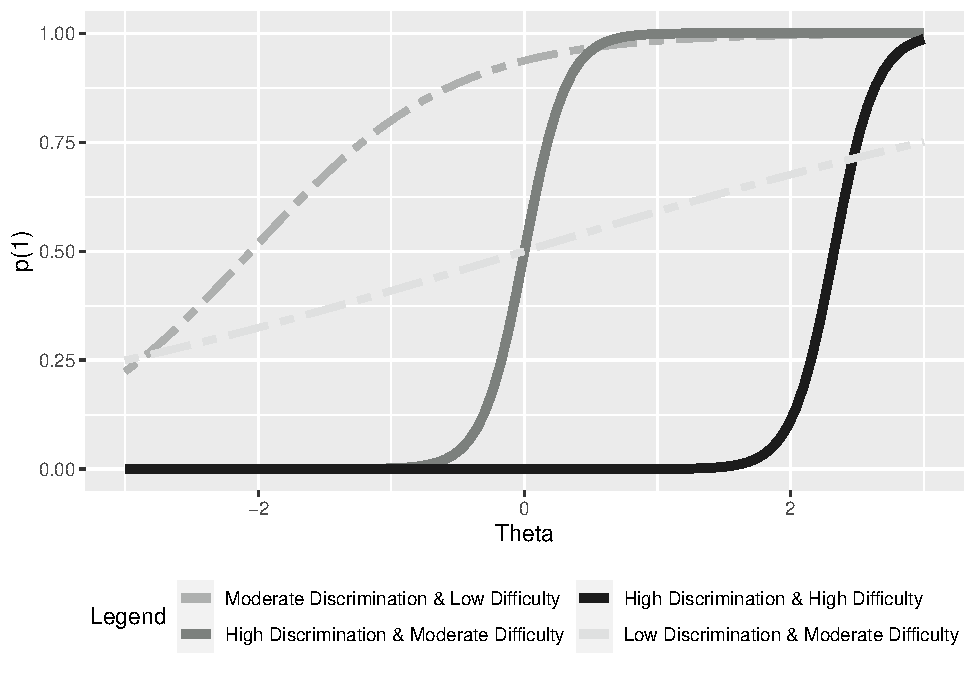
\includegraphics[width=1\linewidth,height=0.8\textheight]{SIOP22_Submission_files/figure-latex/example-1} \caption{Item characteristic curves reflecting differences in difficulty and discrimination.}\label{fig:example}
\end{figure}

Item characteristic curves are frequently consulted by psychometricians as visual indicators of important attributes of assessment items - most commonly \emph{difficulty} and \emph{discrimination}. Within these visual presentations the x-axis ranges along ``trait'' levels (by convention typically denoted with the greek \(\theta\)), whereas the y-axis displays probabilities of responding to the item within a given response category. In the context of true tests, the response categories are binary\footnote{With exception (see, for example, Masters, 1982; Muraki, 1997)}, and the y-axis probability reflects the likelihood of a ``correct'' response\footnote{Because the historical convention in test response is to code a correct response as ``1'' and an incorrect response as ``0'', the y-axis is commonly denoted as ``\emph{p(1)}'' or ``\emph{p(1.0)}''.}. From this visualization, the observer extracts the relationship between a respondent's trait level and the expectation of answering the item correctly. If the curve transitions from low to high likelihood at a location toward the lower end of the trait (e.g., ``left'' on the plotting surface), this indicates that it is relatively easy to answer the item correctly. Stated in the parlance of IRT or Rasch traditions, it does not take much \(\theta\) to have a high likelihood of answering correctly. On the contrary, if the growth in the curve occurs primarily at higher trait levels, this indicates that the item is relatively more difficult. Through the lens of IRT, if discrimination is modeled and the curve is sharp (e.g., strongly vertical), this indicates high discrimination; if it is flatter, that is an indication of poorer discrimination (see Figure \ref{fig:example}).

Assessment specialists who consult ICC's usually do so from within the psychometric framework of either Item Response Theory (IRT) or Rasch modeling. These frameworks estimate the parameters necessary to plot the ogive functions. Rasch models only estimate difficulty, and assume that differences in discrimination represent flaws in measurement. The IRT 2 parameter logistic model (2PL), however, estimates item discrimination in addition to item difficulty. Item difficulty (the \emph{b}-parameter) is scaled as the trait level associated with a 50\% likelihood of correct response (e.g., it is scaled to \(\theta\)). Item discrimination (\emph{a}-parameter) is the degree to which an item differentiates across individuals who are characterized as being relatively lower or higher on the trait. From a Classical Test Theory (CTT) orientation, item difficulty is most commonly represented by the percent of individuals answering the item correctly (also referred to as a \emph{p-value}). Item discrimination can be conveyed via a few different CTT indices, but the most commonly calculated and consulted index is the corrected item-total correlation.

Assessment specialists who calculate these CTT item indices don't typically (to our limited knowledge!) attempt to represent them visually, as is common in IRT and Rasch applications. However, ICC's based on CTT indices could possibly provide snapshot psychometric information as valuable as those gained from IRT- or Rasch-derived item parameters. The largest obstacle to psychometricians deeming CTT-derived visuals to be of value is likely tied to the concept of invariance, which refers to IRT parameter independence across item and person estimates. However, this property is often overstated, as invariance is only attained with perfect model-data fit (which never occurs), and is also only true after being subjected to linear transformation - commonly across samples (Rupp \& Zumbo, 2006). Additionally, several comparative investigations have noted commonality between IRT and CTT difficulty and discrimination estimates as well as relative stability of CTT estimates when samples are large and/or judisciously constructed (Fan, 1998). Fan in fact summarizes that the IRT and CTT frameworks ``\ldots produce very similar item and person statistics'' (p.379). Hambleton and Jones (1993) state that ``no study provides enough empirical evidence on the extent of disparity between the two frameworks and the superiority of IRT over CTT despite the theoretical differences''.

\hypertarget{nature-of-relationship-between-irt-and-ctt-indices}{%
\subsection{Nature of Relationship between IRT and CTT Indices}\label{nature-of-relationship-between-irt-and-ctt-indices}}

F. Lord (1980) described a function that approximates the nonlinear relationship between the IRT \emph{a}-parameter and the CTT discrimination index\footnote{F. Lord (1980)'s CTT discrimination index is actually the item-test biserial correlation as opposed to the contemporarily more popular \emph{corrected} item-total \emph{point-biserial} correlation.}:

\[a_i\cong \frac{r_i}{\sqrt{1-r_i^2}}\]

This formula wasn't intended for practical purposes but rather was specified in an attempt to help assessment specialists who were more familiar with CTT procedures to better understand the relationship to the IRT discrimination parameter. In an effort to move from the conceptual to a practical application, Kulas et al. (2017) proposed a modification that minimized the average residual (either \(a_i\) or \(r_i\), where \(r_i\) is the \emph{corrected} item-total \emph{point-biserial} correlation).

An adjustment to F. M. Lord (2012)'s formula giving the functional relationship between the ``non-invariant'' CTT and ``invariant'' IRT statistics becomes useful in comparing the two methodologies, despite the supposed lack of invariance from CTT. So even though here we acknowledge that invariance is a categorical IRT property, we still follow the functional modification proposed by Kulas et al. (2017), noting that having a large sample that is truly random and whose items are normally distributed and have a center at the moderate difficulty can help reduce threats to CTT ``invariance''.

The Kulas et al. (2017) investigations (both simulated and utilizing real-world test data) identified systematic predictive differences across items with differing item difficulty values, so their recommended formula included a specification for item difficulty (this formulaic specification is also retained in the current presentation):

\[\hat{a_i}\cong[(.51 + .02z_g + .3z_g^2)r]+[(.57 - .009z_g + .19z_g^2)\frac{e^r-e^{-r}}{e-e^r}]\]

\begin{figure}
\centering
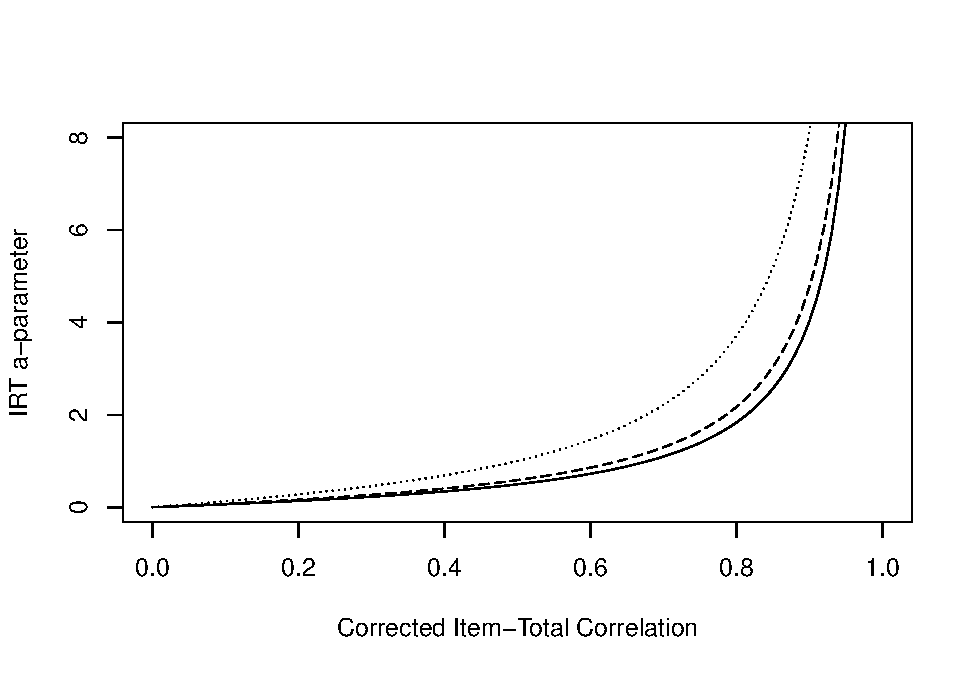
\includegraphics{SIOP22_Submission_files/figure-latex/acorrected-1.pdf}
\caption{\label{fig:acorrected}Empricially-derived functional relationship between the IRT \emph{a} parameter and the CTT corrected-item total correlation as a function of item difficulty (p-value; solid = .5, dashed = .3/.7, dotted = .1/.9).}
\end{figure}

Where \(g\) is the absolute deviation from 50\% responding an item correctly and 50\% responding incorrectly (e.g., a ``p-value'' of .5). \(z_g\) is the standard normal deviate associated with \(g\). This transformation of the standard p-value was recommended in order to scale this index along an interval-level metric more directly analogous to the IRT \emph{b}-parameter. Figure \ref{fig:acorrected} visualizes the re-specifications of Lord's formula at p-values (difficulty) of .5, .3 (or .7), and .1 (or .9) and highlights the nonlinear nature of this relationship - especially noticeable at high(er) levels of discrimination.

As we can see, the higher the corrected item-total correlations, the higher the estimated IRT a-parameter (discrimination). Also, as the p-values (difficulty) deviates from 0, the relationship between the estimated IRT a-parameter and the corrected item-total correlations becomes stronger.

Practitioners and researchers that don't use IRT or Rasch models and instead opt to follow a CTT philosophy would benefit from having ICC's that use CTT statistics. According to Figueiras (2022), they used simulated data to test the overlapping nature of CTT statistics and IRT parameters when plotting ICCs. They used the WinGen program (Han, 2007) and got a sample of 10,000 observations, with a mean of 0 and a standard deviation of 1. The number of items were 100, with response categories of either correct or incorrect (1 and 0). The mean for the a-parameter for the simulated data was 2, and the standard deviation 0.8. The mean for the b-parameter was 0 and the standard deviation 0.5. The mirt package from Chalmers (2012) was used to compute the IRT a-parameters and to plot the 2PL resulting model. As for the CTT-derived a-parameter, the modification to F. M. Lord (2012)'s formula described earlier was used, as well as the re-scaling for the p-values. They additionally changed the scale of the difficulty estimates of CTT so they were on the same scale as the IRT estimates. This was done by building a regression model using the CTT a-estimate to predict the IRT a-parameter. The resulting values from this model were used in plotting the CTT-derived ICC's. When they computed the differences between curves plotted by using IRT estimates and these CTT-derived statistics for all 100 items, they got an average of 0.76.

This study intends to build upon Figueiras (2022)'s work by also looking at differences between ICCs plotted using either IRT or CTT, but this time further modifying the scale of the CTT difficulty estimate. Instead of re-escaling using the regression coefficients estimated from a single IRT simulation, we decided to use five different types of IRT simulations that varied in the shape of their p-value distributions; this is: uniform, normal, inverted, and skewed. Our hypothesis is that the regression slopes of these different conditions will be very similar compared to themselves and that of (\textbf{Figueiras2022items?}) and, in consequence, the areas between the curves of IRT and CTT curves will be the same or smaller after this re-scaling, showing that the overlapping nature of ICCs plotted using IRT and CTT parameters isn't sample dependent.

\hypertarget{study-1}{%
\section{Study 1}\label{study-1}}

Establishing relationship between the IRT and CTT difficulty indices.

\hypertarget{method}{%
\subsection{Method}\label{method}}

Although the ogives could be specified directly from the CTT-derived statistics, we made a procedural decision to retain the IRT 2PL as our function specification:

\[P(\Theta)=\frac{1}{1+e^{-1.7a(\Theta-b)}}\]
Our procedure therefore required the estimation of ``pseudo'' IRT parameters from the CTT indices. The \emph{a} parameter was estimated via the formula specified in Kulas et al. (2017), while the \emph{b} parameter was estimated via linking parameters identified via simulation.

In order to estimate the relationship, we simulated items. We used 100 items and generated 5 different distributions of the p-values of the items. The first distribution was uniform, with the p-values all being different, ranging from 0.1 to 0.99. The third distribution was a normal distribution of p-values, centered around 0.5. The fourth distribution was an inverted normal distribution also centered around 0.5. The fifth distribution was a left skewed distribution of p-values, and the sixth was right skewed.

Then we computed regressions predicting the b-parameters using the standard normal deviate associated with the p-values on each simulation.

\begin{figure}
\centering
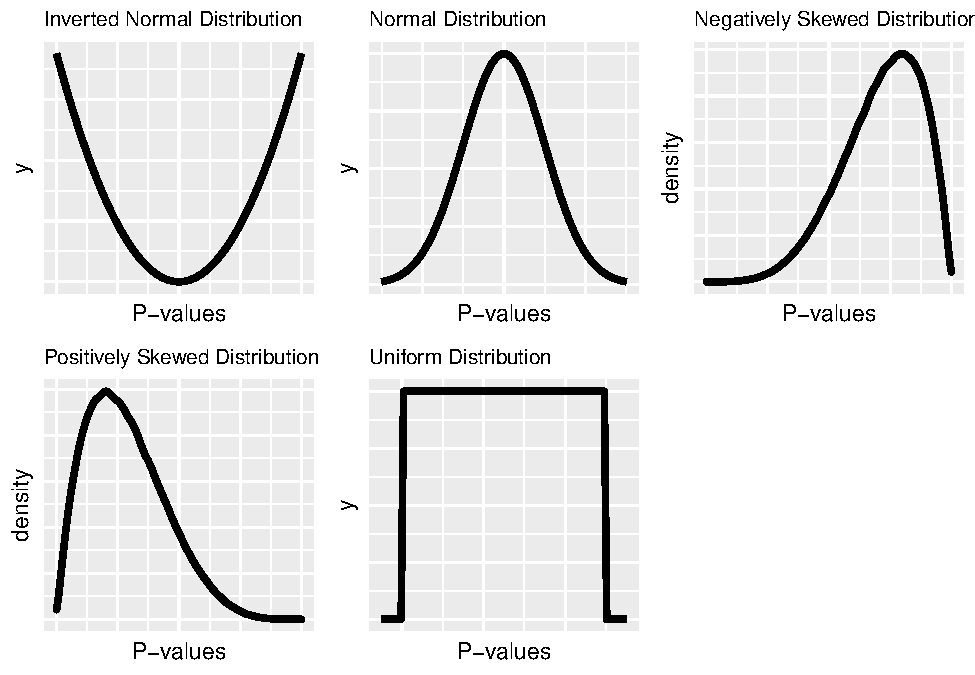
\includegraphics{SIOP22_Submission_files/figure-latex/simulatedgraphs-1.pdf}
\caption{\label{fig:simulatedgraphs}Shape of simulated distributions.}
\end{figure}

\hypertarget{procedure-and-methods}{%
\subsection{Procedure and methods}\label{procedure-and-methods}}

We built six simulations of IRT data using Nydick (2022), each with different shapes and p-values, as can be seen in figure \ref{fig:simulatedgraphs}. Our goal was to see if CTT statistics and IRT parameters would produce similar ICCs when simulated data of varying distributions are used. Each simulation consisted of 10,000 observations and 100 items. Simulation 1 was uniform, with p-values ranging from 0 to 1. Simultion 2 was a normal distribution with p-values centered around 0.5. Simulation 3 was an inverted U-shaped distribution, with p-values ranging from 0 to 1. Simulation 4 was a left skewed distribution with p-values centered around 0.5, and simulation 5 was a right skewed distribution with p-values centered around 0.5.All simulated distributions had an average a-estimate of 1.42 and average b-estimate of 0.5. We ran each simulation 1,000 times, each with 100 items and 10,000 cases.

\hypertarget{results}{%
\subsection{Results}\label{results}}

As shown by figure \ref{fig:acorrected}, our plot looks very similar to that of (Kulas et al., 2017, p. 8). This confirms that our formula for computing the estimated a-parameter follows the exponential relationship we can see in (Kulas et al., 2017; F. M. Lord, 2012).
The resulting regression coefficients for all 5 simulations was an intercept of approximately 0 and a slope of -1.53, indicating that our scaling was not sample dependent, as can be seen in figure \ref{fig:slopes}. In this graph we report the distribution of slopes for all 1,000 simulations per simulation condition. They are all center are about -1.53, with very little deviance in terms of shape, kurtosis, or spread. There were 3,383 cases removed from the overall 500,000 simulated items due to extreme b-estimates.

\begin{figure}
\centering
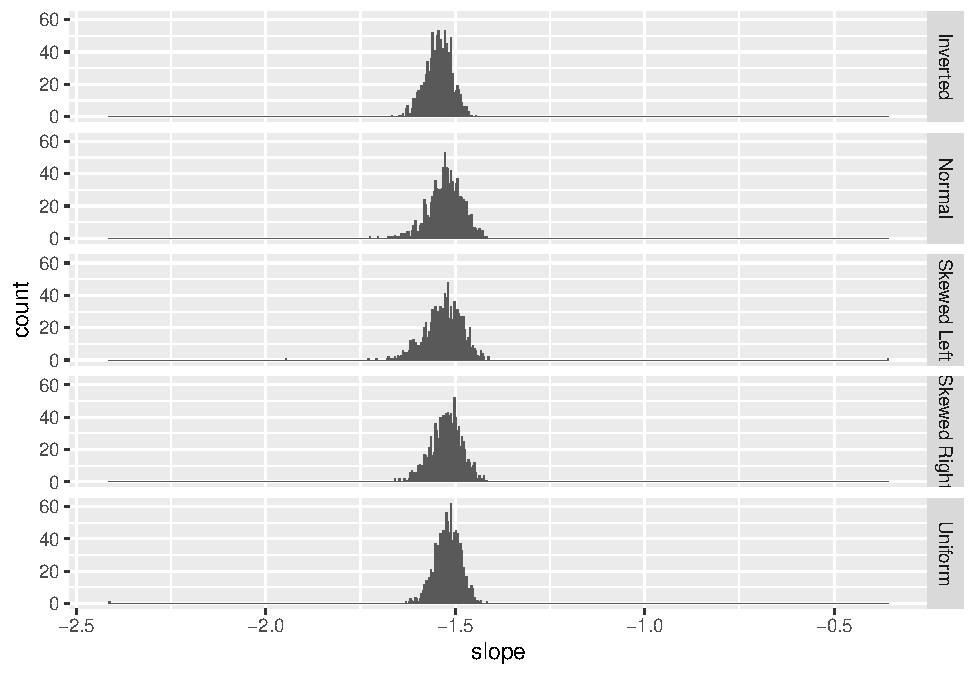
\includegraphics{SIOP22_Submission_files/figure-latex/slopes-1.pdf}
\caption{\label{fig:slopes}Distribution of slopes for 1,000 simulation ran by condition}
\end{figure}

\begin{figure}
\centering
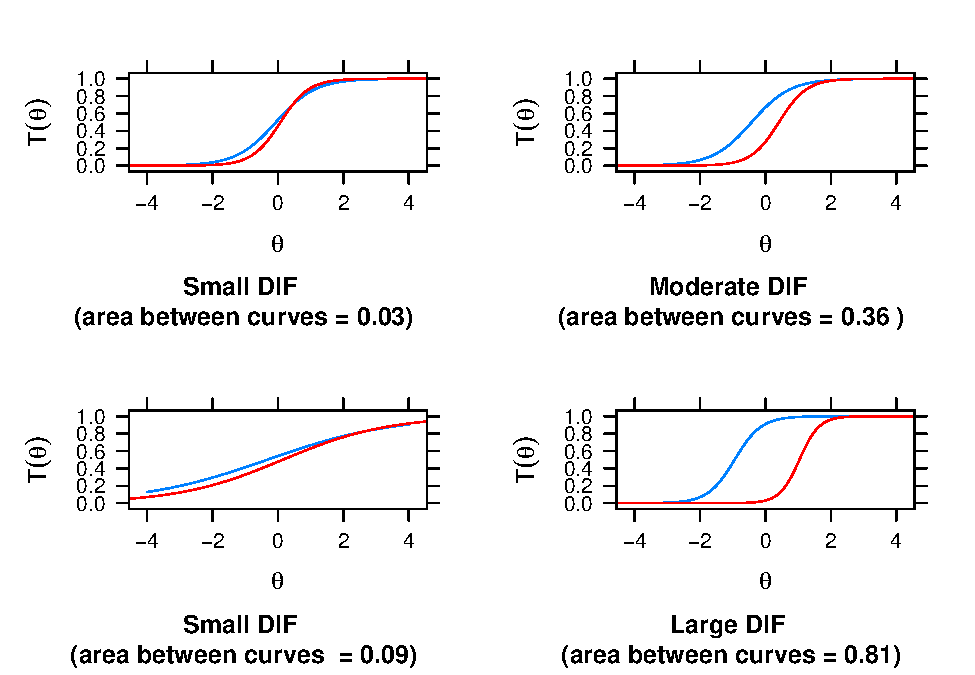
\includegraphics{SIOP22_Submission_files/figure-latex/plotting-1.pdf}
\caption{\label{fig:plotting}Four ICCs highlighting the difference between CTT and IRT-derivated ICCs at different levels of DIF.}
\end{figure}

\begin{figure}
\centering
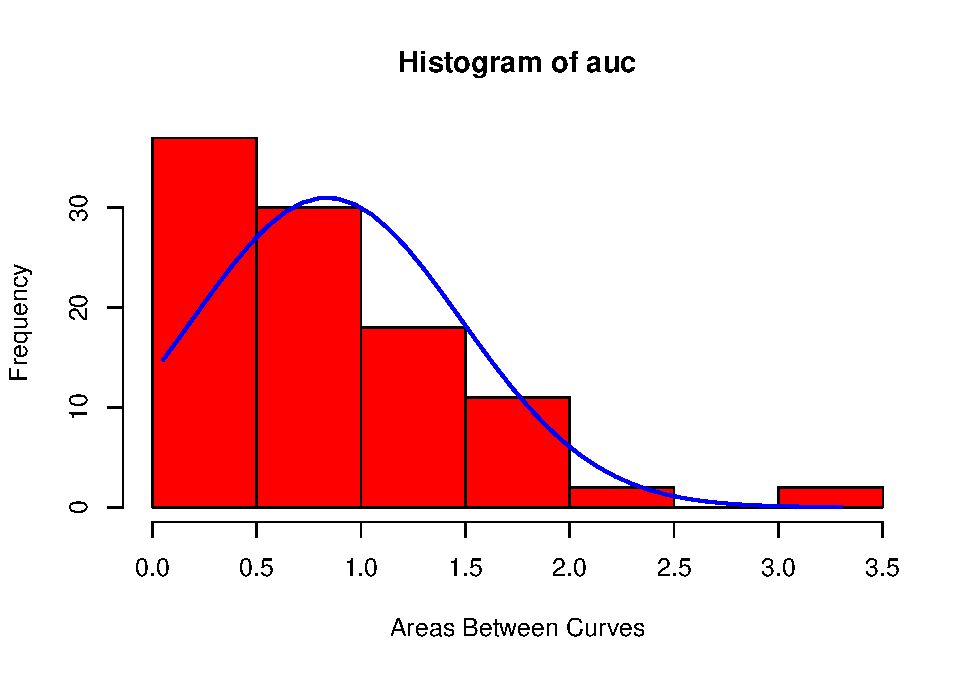
\includegraphics{SIOP22_Submission_files/figure-latex/histrogram-1.pdf}
\caption{\label{fig:histrogram}Histogram of all areas between ICCs plotted using IRT parameters vs ICCs plotted using CTT parameters. The graph to the left is plotted without scaling Zg using the regression coefficients specifications from simulated data. The graph to the right is plotted by scaling Zg with these specifications.}
\end{figure}

\hypertarget{study-2---evaluating-the-comparability-of-irt-and-ctt-iccs}{%
\section{Study 2 - Evaluating the Comparability of IRT and CTT ICC's}\label{study-2---evaluating-the-comparability-of-irt-and-ctt-iccs}}

The purpose of study 2 is to simulate test data and generate ICC's based on the IRT model. Then we compare that to our CTT estimates and look at the differences. We hypothesize that, on average, not only there won't be a big difference between the curves plotted with either methodology, but that after our CTT difficulty parameter re-scaling, this difference will remain the same or smaller.

\hypertarget{procedure-and-materials}{%
\subsection{Procedure and materials}\label{procedure-and-materials}}

The same simulated data as in study 1 was used. The mirt package from Chalmers (2012) was used to compute and plot the IRT statistics. As we can see on figure \ref{fig:plotting}, the blue curves were plotted using 2PL IRT parameters (a and b), while the red curves were plotted using CTT parameters (p-values and corrected item-total correlations, re-scaling and modifying them with Kulas et al. (2017) formulas and estimating pseudo-B using the regression model from the 5 simulations). To quantify the degree of difference between the two curves, the Area Between Curves was computed using R. This procedure was done for all 100 items.

\hypertarget{results-1}{%
\subsection{Results}\label{results-1}}

We used R (Version 4.2.1; R Core Team, 2022) and the R-packages \emph{catIrt} (Version 0.5.1; Nydick, 2022), \emph{descr} (Version 1.1.5; Dirk Enzmann et al., 2021), \emph{dplyr} (Version 1.0.9; Wickham, François, et al., 2022), \emph{faux} (Version 1.1.0; DeBruine, 2021), \emph{fGarch} (Version 4021.88; Wuertz et al., 2022), \emph{forcats} (Version 0.5.1; Wickham, 2021), \emph{ggplot2} (Version 3.3.6; Wickham, 2016), \emph{lattice} (Version 0.20.45; Sarkar, 2008; Sarkar \& Andrews, 2022), \emph{latticeExtra} (Version 0.6.30; Sarkar \& Andrews, 2022), \emph{mirt} (Version 1.36.1; Chalmers, 2012), \emph{numDeriv} (Version 2016.8.1.1; Gilbert \& Varadhan, 2019), \emph{papaja} (Version 0.1.1; Aust \& Barth, 2022), \emph{psych} (Version 2.2.5; Revelle, 2022), \emph{purrr} (Version 0.3.4; Henry \& Wickham, 2020), \emph{readr} (Version 2.1.2; Wickham, Hester, et al., 2022), \emph{reticulate} (Version 1.25; Ushey et al., 2022), \emph{scales} (Version 1.2.0; Wickham \& Seidel, 2022), \emph{stringr} (Version 1.4.0; Wickham, 2019), \emph{tibble} (Version 3.1.8; Müller \& Wickham, 2022), \emph{tidyr} (Version 1.2.0; Wickham \& Girlich, 2022), \emph{tidyverse} (Version 1.3.2; Wickham et al., 2019), and \emph{tinylabels} (Version 0.2.3; Barth, 2022) for all our analyses.

The area between ICC's was calculated between CTT-derived and IRT-derived ICC's. The average difference for all 100 curves was 0.21\footnote{\emph{Note}. Did the integral of the difference between the CTT and IRT functions using the ``integrate'' function in the ``stats'' package (base R). Did a test to confirm this accurately reflects the area between curves by creating two curves, one with high discrimination and another with low discrimination, and seeing what the area between curves was using first the geiger package and then base R. Also roughly estimated by hand this diff. Base R seems to be the more accurate method.}. As we can see in figure \ref{fig:histogram}, most of the data is skewed towards the lower end, indicating that out of the 100 items, most of them have areas between the curves of less than 0.21. This diff was computed after scaling our Zg using the coefficients estimated with our simulations.Without the regression coefficient modifier the average area under the curves were 0.80. We ran a test of significance between these two means. Our results are \(t(99) = 11.72\), \(p < .001\).\\
Four random items were selected and plotted in figure \ref{fig:plotting} using IRT and CTT-derived statistics. The blue curves were plotted using a IRT 2PL model, while the red curves were plotted with CTT-derived parameters.

\hypertarget{discussion}{%
\section{Discussion}\label{discussion}}

Important psychometric information can be gathered from ICC's, which are visual indicators typically of difficulty and discrimination. Psychometricians and other assessment specialists usually examine ICC's under the lenses of IRT and Rasch models. From a CTT orientation, item difficulty is most commonly represented by the percent of individuals answering the item correctly (also referred to as a p-value). Item discrimination can be conveyed via a few CTT indices, but the most commonly calculated and consulted index is the corrected item-total correlation. Assessment specialists who consult these CTT parameters don't typically attempt to represent them visually, as is common in IRT and Rasch applications. However, there is perhaps little reason for them not to do so, as ICC's based on CTT parameters could provide snapshot psychometric information as valuable as those gained from IRT- or Rasch-derived ICC's. Here, following Figueiras (2022)'s work, we first propose an application of ICC's with CTT indices, then we simulated data and quantified similarities and discrepancies between the IRT- and CTT-generated ICC's. Our hypothesis was that the Area Between Curves of these different ICC's would not only be small, but remain so (or become even smaller) if the difficulty CTT statistic was re-scaled using regression specifications from 5 IRT simulations that differed in the shape of the distribution of it's items. Area between curves for 100 items was 0.76 on average without re-scaling this statistic, and 0.21 when the res-caling was done. This result indicates that curves plotted with either IRT or CTT parameters show little difference. The nature of both models is mostly overlapping when it comes to plotting visual representations such as ICC's. Even though there was a significant difference in the area between curves before and after re-scaling, this shows that the differences are even smaller after re-scaling, supporting our hypothesis that the shape of the distribution of p-values plays no role in the overlapping nature of ICCs plotted from IRT and CTT parameters. In other words, this relation is not sample dependent. Practitioners and researchers that don't use IRT or Rasch models and instead opt to follow a CTT philosophy would benefit from having ICC's that use CTT statistics.

Of course there is always an intractability between the CTT item-difficulty index and respondent sample ability. The findings of previous comparison studies, however, point to the CTT estimates exhibiting some degree of invariance across respondent samples.

If this general idea is well-received (SIOP members would seem to represent a great barometer!) we would like to stress the CTT ICC's via further and more extensive conditions. That is, are there patterns that help explain CTT ICCs that diverge from their IRT counterparts? Although our simulations did generate a range of item difficulties and discriminations, we have not yet fully explored systematic patterns of extremely difficult/easy items as well as very poorly discriminating items. If patterns emerge, we would like to model predicted discrepancies via incorporating error bars within our visualizations.

Additionally, if there is interest in this general idea we would likely publish our function as a small \texttt{R} package, perhaps to supplement the \texttt{psych} package's ``alpha'' function, which produces corrected item-total correlations as well as p-values within the same output table (e.g., the ``input'' data is already available in tabular format).

\newpage

\hypertarget{references}{%
\section{References}\label{references}}

\begingroup
\setlength{\parindent}{-0.5in}
\setlength{\leftskip}{0.5in}

\hypertarget{refs}{}
\begin{CSLReferences}{1}{0}
\leavevmode\vadjust pre{\hypertarget{ref-R-papaja}{}}%
Aust, F., \& Barth, M. (2022). \emph{{papaja}: {Prepare} reproducible {APA} journal articles with {R Markdown}}. \url{https://github.com/crsh/papaja}

\leavevmode\vadjust pre{\hypertarget{ref-R-tinylabels}{}}%
Barth, M. (2022). \emph{{tinylabels}: Lightweight variable labels}. \url{https://cran.r-project.org/package=tinylabels}

\leavevmode\vadjust pre{\hypertarget{ref-R-mirt}{}}%
Chalmers, R. P. (2012). {mirt}: A multidimensional item response theory package for the {R} environment. \emph{Journal of Statistical Software}, \emph{48}(6), 1--29. \url{https://doi.org/10.18637/jss.v048.i06}

\leavevmode\vadjust pre{\hypertarget{ref-R-faux}{}}%
DeBruine, L. (2021). \emph{Faux: Simulation for factorial designs}. Zenodo. \url{https://doi.org/10.5281/zenodo.2669586}

\leavevmode\vadjust pre{\hypertarget{ref-R-descr}{}}%
Dirk Enzmann, J. Aquino. I. R. source code and/or documentation written by, Schwartz, M., Jain, N., \& Kraft, S. (2021). \emph{Descr: Descriptive statistics}. \url{https://CRAN.R-project.org/package=descr}

\leavevmode\vadjust pre{\hypertarget{ref-fan1998item}{}}%
Fan, X. (1998). Item response theory and classical test theory: An empirical comparison of their item/person statistics. \emph{Educational and Psychological Measurement}, \emph{58}(3), 357--381.

\leavevmode\vadjust pre{\hypertarget{ref-Figueiras2022item}{}}%
Figueiras, K., Diego. (2022). \emph{Item characteristic curve estimation from common classical test theory indices}. SIOP.

\leavevmode\vadjust pre{\hypertarget{ref-R-numDeriv}{}}%
Gilbert, P., \& Varadhan, R. (2019). \emph{numDeriv: Accurate numerical derivatives}. \url{https://CRAN.R-project.org/package=numDeriv}

\leavevmode\vadjust pre{\hypertarget{ref-hambleton1993comparison}{}}%
Hambleton, R. K., \& Jones, R. W. (1993). Comparison of classical test theory and item response theory and their applications to test development. \emph{Educational Measurement: Issues and Practice}, \emph{12}(3), 38--47.

\leavevmode\vadjust pre{\hypertarget{ref-han2007wingen3}{}}%
Han, K. T. (2007). WinGen: Windows software that generates IRT parameters and item responses. \emph{Applied Psychological Measurement}, \emph{31}(5), 457--459.

\leavevmode\vadjust pre{\hypertarget{ref-R-purrr}{}}%
Henry, L., \& Wickham, H. (2020). \emph{Purrr: Functional programming tools}. \url{https://CRAN.R-project.org/package=purrr}

\leavevmode\vadjust pre{\hypertarget{ref-kulas2017approximate}{}}%
Kulas, J. T., Smith, J. A., \& Xu, H. (2017). Approximate functional relationship between IRT and CTT item discrimination indices: A simulation, validation, and practical extension of {Lord's} (1980) formula. \emph{Journal of Applied Measurement}, \emph{18}(4), 393--407.

\leavevmode\vadjust pre{\hypertarget{ref-lord1980applications}{}}%
Lord, F. (1980). \emph{Applications of IRT to practical problems}. Hillsdale: Lawrence Erlbaum Associates.

\leavevmode\vadjust pre{\hypertarget{ref-lord2012applications}{}}%
Lord, F. M. (2012). \emph{Applications of item response theory to practical testing problems}. Routledge.

\leavevmode\vadjust pre{\hypertarget{ref-masters1982rasch}{}}%
Masters, G. N. (1982). A rasch model for partial credit scoring. \emph{Psychometrika}, \emph{47}(2), 149--174.

\leavevmode\vadjust pre{\hypertarget{ref-R-tibble}{}}%
Müller, K., \& Wickham, H. (2022). \emph{Tibble: Simple data frames}. \url{https://CRAN.R-project.org/package=tibble}

\leavevmode\vadjust pre{\hypertarget{ref-muraki1997generalized}{}}%
Muraki, E. (1997). A generalized partial credit model. In \emph{Handbook of modern item response theory} (pp. 153--164). Springer.

\leavevmode\vadjust pre{\hypertarget{ref-R-catIrt}{}}%
Nydick, S. (2022). \emph{catIrt: Simulate IRT-based computerized adaptive tests}. \url{https://CRAN.R-project.org/package=catIrt}

\leavevmode\vadjust pre{\hypertarget{ref-R-base}{}}%
R Core Team. (2022). \emph{R: A language and environment for statistical computing}. R Foundation for Statistical Computing. \url{https://www.R-project.org/}

\leavevmode\vadjust pre{\hypertarget{ref-R-psych}{}}%
Revelle, W. (2022). \emph{Psych: Procedures for psychological, psychometric, and personality research}. Northwestern University. \url{https://CRAN.R-project.org/package=psych}

\leavevmode\vadjust pre{\hypertarget{ref-rupp2006understanding}{}}%
Rupp, A. A., \& Zumbo, B. D. (2006). Understanding parameter invariance in unidimensional IRT models. \emph{Educational and Psychological Measurement}, \emph{66}(1), 63--84.

\leavevmode\vadjust pre{\hypertarget{ref-R-lattice}{}}%
Sarkar, D. (2008). \emph{Lattice: Multivariate data visualization with r}. Springer. \url{http://lmdvr.r-forge.r-project.org}

\leavevmode\vadjust pre{\hypertarget{ref-R-latticeExtra}{}}%
Sarkar, D., \& Andrews, F. (2022). \emph{latticeExtra: Extra graphical utilities based on lattice}. \url{https://CRAN.R-project.org/package=latticeExtra}

\leavevmode\vadjust pre{\hypertarget{ref-R-reticulate}{}}%
Ushey, K., Allaire, J., \& Tang, Y. (2022). \emph{Reticulate: Interface to 'python'}. \url{https://CRAN.R-project.org/package=reticulate}

\leavevmode\vadjust pre{\hypertarget{ref-R-ggplot2}{}}%
Wickham, H. (2016). \emph{ggplot2: Elegant graphics for data analysis}. Springer-Verlag New York. \url{https://ggplot2.tidyverse.org}

\leavevmode\vadjust pre{\hypertarget{ref-R-stringr}{}}%
Wickham, H. (2019). \emph{Stringr: Simple, consistent wrappers for common string operations}. \url{https://CRAN.R-project.org/package=stringr}

\leavevmode\vadjust pre{\hypertarget{ref-R-forcats}{}}%
Wickham, H. (2021). \emph{Forcats: Tools for working with categorical variables (factors)}. \url{https://CRAN.R-project.org/package=forcats}

\leavevmode\vadjust pre{\hypertarget{ref-R-tidyverse}{}}%
Wickham, H., Averick, M., Bryan, J., Chang, W., McGowan, L. D., François, R., Grolemund, G., Hayes, A., Henry, L., Hester, J., Kuhn, M., Pedersen, T. L., Miller, E., Bache, S. M., Müller, K., Ooms, J., Robinson, D., Seidel, D. P., Spinu, V., \ldots{} Yutani, H. (2019). Welcome to the {tidyverse}. \emph{Journal of Open Source Software}, \emph{4}(43), 1686. \url{https://doi.org/10.21105/joss.01686}

\leavevmode\vadjust pre{\hypertarget{ref-R-dplyr}{}}%
Wickham, H., François, R., Henry, L., \& Müller, K. (2022). \emph{Dplyr: A grammar of data manipulation}. \url{https://CRAN.R-project.org/package=dplyr}

\leavevmode\vadjust pre{\hypertarget{ref-R-tidyr}{}}%
Wickham, H., \& Girlich, M. (2022). \emph{Tidyr: Tidy messy data}. \url{https://CRAN.R-project.org/package=tidyr}

\leavevmode\vadjust pre{\hypertarget{ref-R-readr}{}}%
Wickham, H., Hester, J., \& Bryan, J. (2022). \emph{Readr: Read rectangular text data}. \url{https://CRAN.R-project.org/package=readr}

\leavevmode\vadjust pre{\hypertarget{ref-R-scales}{}}%
Wickham, H., \& Seidel, D. (2022). \emph{Scales: Scale functions for visualization}. \url{https://CRAN.R-project.org/package=scales}

\leavevmode\vadjust pre{\hypertarget{ref-R-fGarch}{}}%
Wuertz, D., Chalabi, Y., Setz, T., \& Maechler, M. (2022). \emph{fGarch: Rmetrics - autoregressive conditional heteroskedastic modelling}. \url{https://CRAN.R-project.org/package=fGarch}

\end{CSLReferences}

\endgroup


\end{document}
